\documentclass[10pt]{article}
\usepackage{amsmath}
\usepackage{amsthm}
\usepackage{amsfonts}
\usepackage{amssymb}
\usepackage{amssymb}
\usepackage{booktabs}
\setlength\parindent{0pt}
\usepackage[margin=1.2in]{geometry}
\usepackage{enumitem}
\usepackage{mathtools}
\mathtoolsset{showonlyrefs=true}
\usepackage{pdflscape}
\usepackage{xcolor}
\usepackage{hyperref}
\setcounter{tocdepth}{4}
\setcounter{secnumdepth}{4}
\usepackage[listings,skins,breakable]{tcolorbox} % package for colored boxes
\usepackage{etoolbox}
\usepackage{placeins}
\usepackage{tikz}
\usepackage{color}  % Allows for color customization
\usepackage{subcaption}
\usepackage[utf8]{inputenc}


% Make it so that the bottom page of a 
% book section doesn't have weird spacing
\raggedbottom


% Define custom colors
% You can-redo these later, they're not being used 
% for anything as of 5/12/24
\definecolor{codegreen}{rgb}{0,0.6,0}
\definecolor{codegray}{rgb}{0.5,0.5,0.5}
\definecolor{codepurple}{rgb}{0.58,0,0.82}
\definecolor{backcolour}{rgb}{0.95,0.95,0.92}

% You can-redo the lstlisting style later, it's not being used 
% for anything as of 5/12/24

% Define the lstlisting style
\lstdefinestyle{mystyle}{
    backgroundcolor=\color{backcolour},   
    commentstyle=\color{codegreen},
    keywordstyle=\color{magenta},
    numberstyle=\tiny\color{codegray},
    stringstyle=\color{codepurple},
    basicstyle=\ttfamily\footnotesize,
    breakatwhitespace=false,         
    breaklines=true,                 
    captionpos=b,                    
    keepspaces=true,                 
    numbers=left,                    
    numbersep=5pt,                  
    showspaces=false,                
    showstringspaces=false,
    showtabs=false,                  
    tabsize=2
}
\lstset{style=mystyle}


% Set the length of \parskip to add a line between paragraphs
\setlength{\parskip}{1em}


% Set the second level of itemize to use \circ as the bullet point
\setlist[itemize,2]{label={$\circ$}}

% Define symbols
\DeclareMathSymbol{\Perp}{\mathrel}{symbols}{"3F}
\newcommand\barbelow[1]{\stackunder[1.2pt]{$#1$}{\rule{.8ex}{.075ex}}}
\newcommand{\succprec}{\mathrel{\mathpalette\succ@prec{\succ\prec}}}
\newcommand{\precsucc}{\mathrel{\mathpalette\succ@prec{\prec\succ}}}


\newcounter{example}[section] % Reset example counter at each new section
\renewcommand{\theexample}{\thesection.\arabic{example}} % Format the example number as section.number

\newenvironment{example}
  {% Begin environment
   \refstepcounter{example}% Step counter and allow for labeling
   \noindent\textbf{Example \theexample.} % Display the example number
  }
  {% End environment
   \par\noindent\hfill\textit{End of Example.}\par
  }



% deeper section command
% This will let you go one level deeper than whatever section level you're on.
\makeatletter
\newcommand{\deepersection}[1]{%
  \ifnum\value{subparagraph}>0
    % Already at the deepest standard level (\subparagraph), cannot go deeper
    \subparagraph{#1}
  \else
    \ifnum\value{paragraph}>0
      \subparagraph{#1}
    \else
      \ifnum\value{subsubsection}>0
        \paragraph{#1}
      \else
        \ifnum\value{subsection}>0
          \subsubsection{#1}
        \else
          \ifnum\value{section}>0
            \subsection{#1}
          \else
            \section{#1}
          \fi
        \fi
      \fi
    \fi
  \fi
}
\makeatother


% same section command
% This will let create a section at the same level as whatever section level you're on.
\makeatletter
\newcommand{\samesection}[1]{%
  \ifnum\value{subparagraph}>0
    \subparagraph{#1}
  \else
    \ifnum\value{paragraph}>0
      \paragraph{#1}
    \else
      \ifnum\value{subsubsection}>0
        \subsubsection{#1}
      \else
        \ifnum\value{subsection}>0
          \subsection{#1}
        \else
          \ifnum\value{section}>0
            \section{#1}
          \else
            % Default to section if outside any sectioning
            \section{#1}
          \fi
        \fi
      \fi
    \fi
  \fi
}
\makeatother

\makeatletter
\newcommand{\shallowersection}[1]{%
  \ifnum\value{subparagraph}>0
    \paragraph{#1} % From subparagraph to paragraph
  \else
    \ifnum\value{paragraph}>0
      \subsubsection{#1} % From paragraph to subsubsection
    \else
      \ifnum\value{subsubsection}>0
        \subsection{#1} % From subsubsection to subsection
      \else
        \ifnum\value{subsection}>0
          \section{#1} % From subsection to section
        \else
          \ifnum\value{section}>0
            \chapter{#1} % Assuming a document class with chapters
          \else
            \section{#1} % Default to section if somehow higher than section
          \fi
        \fi
      \fi
    \fi
  \fi
}
\makeatother



\newcounter{problemcounter}
\renewcommand{\theproblemcounter}{Q.\arabic{problemcounter}}

% Define the problem environment
\newenvironment{problem}[1][]{%
  \refstepcounter{problemcounter}%
  \if\relax\detokenize{#1}\relax
    \tcolorbox[breakable, colback=red!10, colframe=red!50, fonttitle=\bfseries, title={Problem \theproblemcounter}, arc=5mm, boxrule=0.5mm]
  \else
    \tcolorbox[breakable, colback=red!10, colframe=red!50, fonttitle=\bfseries, title={Problem \theproblemcounter: #1}, arc=5mm, boxrule=0.5mm]
    \addcontentsline{toc}{subsubsection}{\theproblemcounter: #1}%
  \fi
}{
  \endtcolorbox
}

% Define a new counter for definitions
\newcounter{definitioncounter}
\renewcommand{\thedefinitioncounter}{D.\arabic{definitioncounter}}

\newenvironment{definition}[1][]{%
  \refstepcounter{definitioncounter}%
  \if\relax\detokenize{#1}\relax
    \tcolorbox[
      breakable,
      parbox=false, % Treat content normally regarding paragraphs
      before upper={\parindent0pt \parskip7pt}, % No indentation and add space between paragraphs
      colback=blue!10,
      colframe=blue!50,
      fonttitle=\bfseries,
      title={Definition \thedefinitioncounter},
      arc=5mm,
      boxrule=0.5mm,
      before skip=10pt, % Adjust vertical space before the box
      after skip=10pt % Adjust vertical space after the box
    ]
  \else
    \tcolorbox[
      breakable,
      parbox=false,
      before upper={\parindent0pt \parskip7pt},
      colback=blue!10,
      colframe=blue!50,
      fonttitle=\bfseries,
      title={Definition \thedefinitioncounter: #1},
      arc=5mm,
      boxrule=0.5mm,
      before skip=10pt,
      after skip=10pt
    ]
  \fi
}{
  \endtcolorbox
}


% Define a new counter for theorems
\newcounter{theoremcounter}
\renewcommand{\thetheoremcounter}{T.\arabic{theoremcounter}}

\newenvironment{theorem}[1][]{%
  \refstepcounter{theoremcounter}%
  \if\relax\detokenize{#1}\relax
    \tcolorbox[
      breakable,
      parbox=false, % Treat content normally regarding paragraphs
      before upper={\parindent0pt \parskip7pt}, % No indentation and add space between paragraphs
      colback=green!10,
      colframe=green!55,
      fonttitle=\bfseries,
      title={Theorem \thetheoremcounter},
      arc=5mm,
      boxrule=0.5mm,
      before skip=10pt, % Adjust vertical space before the box
      after skip=10pt % Adjust vertical space after the box
    ]
  \else
    \tcolorbox[
      breakable,
      parbox=false,
      before upper={\parindent0pt \parskip7pt},
      colback=green!10,
      colframe=green!55,
      fonttitle=\bfseries,
      title={Theorem \thetheoremcounter: #1},
      arc=5mm,
      boxrule=0.5mm,
      before skip=10pt,
      after skip=10pt
    ]
  \fi
}{
  \endtcolorbox
}


% Define a new counter for remarks
\newcounter{remarkcounter}
\renewcommand{\theremarkcounter}{R.\arabic{remarkcounter}}

\newenvironment{remark}[1][]{%
  \refstepcounter{remarkcounter}%
  \if\relax\detokenize{#1}\relax
    \tcolorbox[
      breakable,
      parbox=false, % Treat content normally regarding paragraphs
      before upper={\parindent0pt \parskip7pt}, % No indentation and add space between paragraphs
      colback=green!10,
      colframe=green!55,
      fonttitle=\bfseries,
      title={Remark \theremarkcounter},
      arc=5mm,
      boxrule=0.5mm,
      before skip=10pt, % Adjust vertical space before the box
      after skip=10pt % Adjust vertical space after the box
    ]
  \else
    \tcolorbox[
      breakable,
      parbox=false,
      before upper={\parindent0pt \parskip7pt},
      colback=green!10,
      colframe=green!55,
      fonttitle=\bfseries,
      title={Remark \theremarkcounter: #1},
      arc=5mm,
      boxrule=0.5mm,
      before skip=10pt,
      after skip=10pt
    ]
  \fi
}{
  \endtcolorbox
}

% Define a new counter for lemmas
\newcounter{lemmacounter}
\renewcommand{\thelemmacounter}{L.\arabic{lemmacounter}}

\newenvironment{lemma}[1][]{%
  \refstepcounter{lemmacounter}%
  \if\relax\detokenize{#1}\relax
    \tcolorbox[
      breakable,
      parbox=false, % Treat content normally regarding paragraphs
      before upper={\parindent0pt \parskip7pt}, % No indentation and add space between paragraphs
      colback=green!10,
      colframe=green!55,
      fonttitle=\bfseries,
      title={Lemma \thelemmacounter},
      arc=5mm,
      boxrule=0.5mm,
      before skip=10pt, % Adjust vertical space before the box
      after skip=10pt % Adjust vertical space after the box
    ]
  \else
    \tcolorbox[
      breakable,
      parbox=false,
      before upper={\parindent0pt \parskip7pt},
      colback=green!10,
      colframe=green!55,
      fonttitle=\bfseries,
      title={Lemma \thelemmacounter: #1},
      arc=5mm,
      boxrule=0.5mm,
      before skip=10pt,
      after skip=10pt
    ]
  \fi
}{
  \endtcolorbox
}

% Define a new counter for propositions
\newcounter{propositioncounter}
\renewcommand{\thepropositioncounter}{P.\arabic{propositioncounter}}

\newenvironment{proposition}[1][]{%
  \refstepcounter{propositioncounter}%
  \if\relax\detokenize{#1}\relax
    \tcolorbox[
      breakable,
      parbox=false, % Treat content normally regarding paragraphs
      before upper={\parindent0pt \parskip7pt}, % No indentation and add space between paragraphs
      colback=green!10,
      colframe=green!55,
      fonttitle=\bfseries,
      title={Proposition \thepropositioncounter},
      arc=5mm,
      boxrule=0.5mm,
      before skip=10pt, % Adjust vertical space before the box
      after skip=10pt % Adjust vertical space after the box
    ]
  \else
    \tcolorbox[
      breakable,
      parbox=false,
      before upper={\parindent0pt \parskip7pt},
      colback=green!10,
      colframe=green!55,
      fonttitle=\bfseries,
      title={Proposition \thepropositioncounter: #1},
      arc=5mm,
      boxrule=0.5mm,
      before skip=10pt,
      after skip=10pt
    ]
  \fi
}{
  \endtcolorbox
}

%\newtheorem{proposition}[theorem]{Proposition}  % Propositions share numbering with theorems


% Define a new counter for notes
\newcounter{notescounter}
\renewcommand{\thenotescounter}{D.\arabic{notescounter}}

\newenvironment{notes}[1][]{
  \refstepcounter{notescounter}%
  \if\relax\detokenize{#1}\relax
    % If #1 is empty, set the title to "Notes"
    \tcolorbox[
      breakable,
      parbox=false, % Treat content normally regarding paragraphs
      before upper={\parindent0pt \parskip7pt}, % No indentation and add space between paragraphs
      colback=blue!10,
      colframe=blue!50,
      fonttitle=\bfseries,
      title={Notes},
      arc=5mm,
      boxrule=0.5mm,
      before skip=10pt, % Adjust vertical space before the box
      after skip=10pt % Adjust vertical space after the box
    ]
  \else
    % If #1 is not empty, use it as the title
    \tcolorbox[
      breakable,
      parbox=false,
      before upper={\parindent0pt \parskip7pt},
      colback=blue!10,
      colframe=blue!50,
      fonttitle=\bfseries,
      title={#1}, % Use provided title instead of default
      arc=5mm,
      boxrule=0.5mm,
      before skip=10pt,
      after skip=10pt
    ]
  \fi
}{
  \endtcolorbox
}







% Define a new counter for questions
\newcounter{questionscounter}
\renewcommand{\thequestionscounter}{D.\arabic{questionscounter}}

\newenvironment{questions}[1][]{
  \refstepcounter{questionscounter}%
  \if\relax\detokenize{#1}\relax
    % If #1 is empty, set the title to "Questions"
    \tcolorbox[
      breakable,
      parbox=false, % Treat content normally regarding paragraphs
      before upper={\parindent0pt \parskip7pt}, % No indentation and add space between paragraphs
      colback=red!10,
      colframe=red!50,
      fonttitle=\bfseries,
      title={Questions},
      arc=5mm,
      boxrule=0.5mm,
      before skip=10pt, % Adjust vertical space before the box
      after skip=10pt % Adjust vertical space after the box
    ]
  \else
    % If #1 is not empty, use it as the title
    \tcolorbox[
      breakable,
      parbox=false,
      before upper={\parindent0pt \parskip7pt},
      colback=red!10,
      colframe=red!50,
      fonttitle=\bfseries,
      title={#1}, % Use provided title instead of default
      arc=5mm,
      boxrule=0.5mm,
      before skip=10pt,
      after skip=10pt
    ]
  \fi
}{
  \endtcolorbox
}






% Define a new counter for overview
\newcounter{overviewcounter}
\renewcommand{\theoverviewcounter}{D.\arabic{overviewcounter}}

\newenvironment{overview}[1][]{%
  \refstepcounter{overviewcounter}%
  \if\relax\detokenize{#1}\relax
    \tcolorbox[
      breakable,
      parbox=false, % Treat content normally regarding paragraphs
      before upper={\parindent0pt \parskip7pt}, % No indentation and add space between paragraphs
      colback=green!10,
      colframe=green!55,
      fonttitle=\bfseries,
      title={Overview},
      arc=5mm,
      boxrule=0.5mm,
      before skip=10pt, % Adjust vertical space before the box
      after skip=10pt % Adjust vertical space after the box
    ]
  \else
    \tcolorbox[
      breakable,
      parbox=false,
      before upper={\parindent0pt \parskip7pt},
      colback=green!10,
      colframe=green!55,
      fonttitle=\bfseries,
      title={Overview},
      arc=5mm,
      boxrule=0.5mm,
      before skip=10pt,
      after skip=10pt
    ]
  \fi
}{
  \endtcolorbox
}



% Add a line after paragraph header
\makeatletter
\renewcommand\paragraph{\@startsection{paragraph}{4}{\z@}%
            {-3.25ex \@plus -1ex \@minus -.2ex}%
            {1.5ex \@plus .2ex}%
            {\normalfont\normalsize\bfseries}}
\makeatother


% Taking away line before and after align
\BeforeBeginEnvironment{align}{\vspace{-\parskip}}
\AfterEndEnvironment{align}{\vskip0pt plus 2pt}

\usepackage{changepage}

\title{Ch. 9: Experiments with Longitudinal Elements}

\author{Dylan Baker}

\begin{document}
\maketitle

\tableofcontents


\section{Main Takeaways}

\subsection{Gains from Pre-Treatment Outcome Measures}

Consider the two parameters:

\begin{align}
        \tau^{D I D}=\tau^{\text {post }} & -\tau^{\text {pre }} \\
        = & \sum_{t>0}\left(\mathbb{E}\left[Y_{i t} \mid D_{i t}=1\right]-\mathbb{E}\left[Y_{i t} \mid D_{i t}=0\right]\right) \\
        & -\sum_{t \leq 0}\left(\mathbb{E}\left[Y_{i t} \mid D_{i t}=1\right]-\mathbb{E}\left[Y_{i t} \mid D_{i t}=0\right]\right)
\end{align}

and

\begin{align}
    \tau^{\text {Post }}=\sum_{t>0}\left(\mathbb{E}\left[Y_{i t} \mid D_{i t}=1\right]-\mathbb{E}\left[Y_{i t} \mid D_{i t}=0\right]\right)
\end{align}

When you have pre-treatment observations, there are instances 
where it may be beneficial to include them in your specification 
and instances where it may not be. This depends on how many 
pre-treatment observations you have and the strength of the 
autocorrelation parameter.

Under the assumptions of 
\begin{enumerate}
    \item constant variance across time periods, 
    \item equal variances between all pairs of time points
    \item autocorrelation in outcomes does not depend on treatment effects
    \item treatment and control groups are identical in cross-sectional size
\end{enumerate}

we have 

\begin{align}
    \operatorname{Var}\left[\tau^{\text {Post }}\right]=\frac{2 \sigma^2}{n_d}\left(\frac{1+\left(N_{\text {Post }}-1\right) \rho}{N_{\text {Post }}}\right)
\end{align}

and 

\begin{align}
    \operatorname{Var}\left[\tau^{D I D}\right]=\frac{2 \sigma^2}{n_d}\left(\frac{1+\left(N_{\text {Post }}-1\right) \rho}{N_{\text {Post }}}-\frac{\left(N_{\text {Pre }}+1\right) \rho-1}{N_{\text {Pre }}}\right)
\end{align}

Below is a guide:

\begin{figure}[!htb]
    \centering
        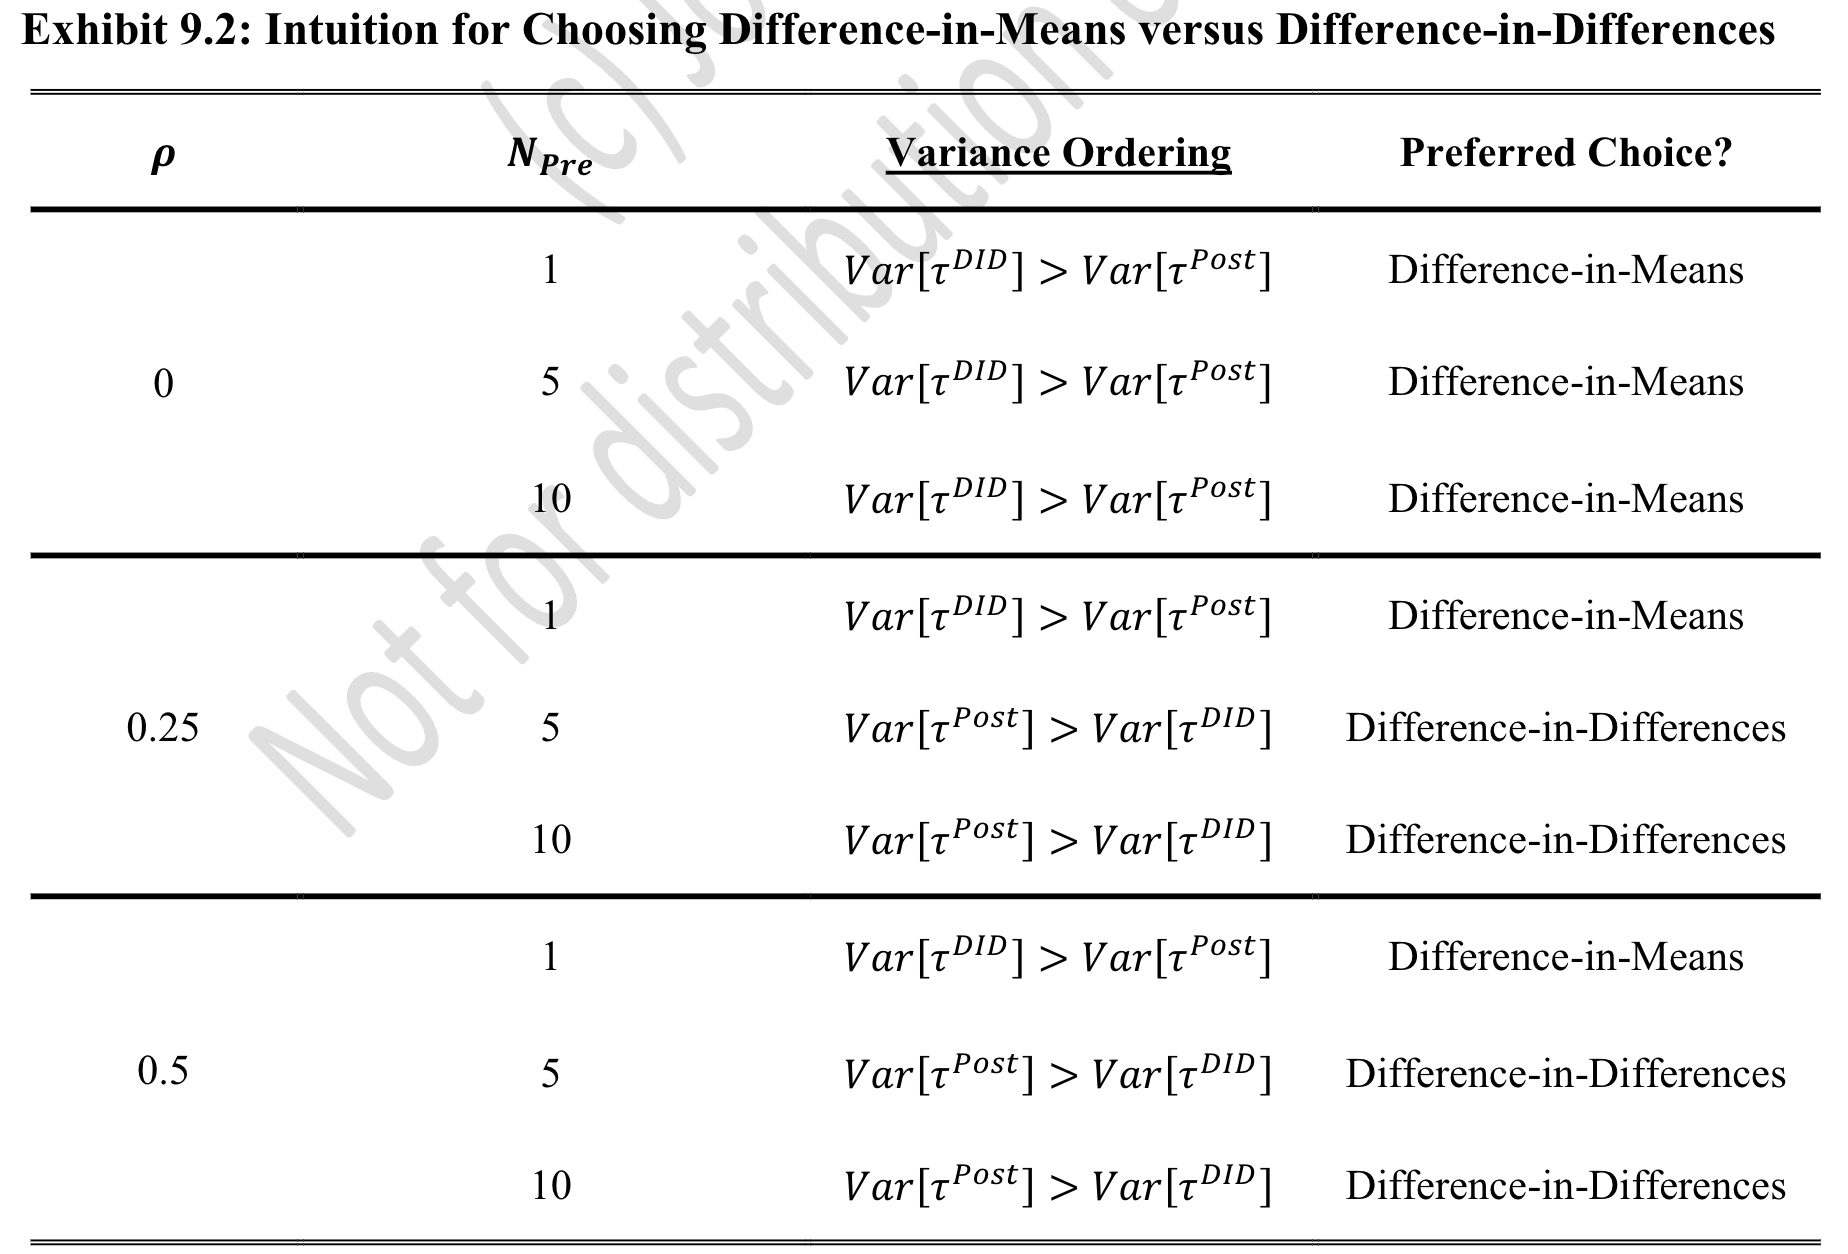
\includegraphics[width=0.6\textwidth]{../input/simple_mean_v_diff_diff.png}
    \caption{Choosing Diff-in-Diff versus Diff-in-Means}
    %\label{fig:}
\end{figure}

\subsection{Choosing the Optimal Number of Pre- and Post- Periods}

The smallest sample size correspond to a 
given MDE is given by:

\begin{align}
    n_0^*=n_1^*=n^*=\frac{2\left(t_{\alpha / 2}+t_\beta\right)^2 \sigma^2}{(M D E)^2}\left(\frac{N_{\text {Pre }}+N_{\text {Post }}}{N_{\text {Pre }} * N_{\text {Post }}}\right)
\end{align}

As the number of periods increases from 4 to 16, the 
minimum sample size required to detect a given MDE
decreases four-fold.

\begin{questions}
    Look into this more.
\end{questions}


\subsection{Solomon 4-Group Design}

One may worry that taking measures repeatedly 
may influence participants' responses (e.g., if they 
get tired of responding). One way to get around this 
is to use the Solomon 4-group design. Under this design,
participants are randomly divided into to 2, where 
half are given a pre-test and half are not. Then,
post-test outcomes are measured for all participants
and compared based on whether they received a pre-test. 
If results are similar across groups, they can be pooled.


\subsection{Causal Density}


``The actual measurement of a long run treatment effect and the discovered underlying 
mechanisms at work depends on the outcome's causal density.

The causal density of an outcome variable refers to how well the 
determinants of the outcome are understood. An outcome with low 
causal density is one where the factors determining the outcome 
are well understood. For example, farmers have a near-perfect 
understanding of the determinants of crop yields, yielding a low 
causal density. In contrast, the determinants of labor market 
outcomes are much less well understood and thus have high causal density. 
For example, future employment and wage outcomes are a function 
of the numerous and interconnected inputs by multiple people 
and institutions.''

``As the time between experiment and observation of the outcome increases, 
so do the number of potential mechanisms driving the effect and
the causal density. For example, consider the question of 
whether financial incentives increase test scores. Suppose 
the researcher announces the incentives right before 
she administers the test. In that case, one can be 
reasonably sure that the only mechanism through which the
treatment works is the student's effort on the test. 
Conversely, suppose that the researcher announces the 
financial incentives months before administering the test.
Then, the student's effort remains a potential mechanism.
However, possible changes to the student's test score
could arise through her own study effort or even investment
rom her parents, teachers, or peers. This general
problem is one of forecasting long-term treatment outcomes, 
and its applicability is quite widespread.''

\subsection{Surrogates}

When we are interested in the long-run effect of something 
but may be interested in expanding the policy before we 
can observe the long-run effect, we may use a surrogate
to estimate the long-run effect. In this case, under strong assumptions,
we consider the effect of the treatment on the surrogate
and the effect of the surrogate on the long-run outcome.

The key assumptions are:

\begin{notes}
    \begin{enumerate}
        \item (A9.3, Comparability): $P_i \perp Y_i \mid Y_i^S$
            \begin{itemize}
                \item That is, 
                    the ``conditional distribution of the primary 
                    outcome given the surrogates is the
                    same in the observational and experimental samples.''
            \end{itemize}
        \item A linear relationship between the outcome and the surrogate
        \item $\text{Var}\left[Y_i^S \mid D_i\right]=\text{Var}\left[Y_i \mid D_i\right]$
        \item (A9.4, Surrogacy Condition): $D_i \perp Y_i \mid Y_i^S$
            \begin{itemize}
                \item ``The surrogacy condition requires that the surrogate 
                fully captures the causal link between the treatment and 
                the primary outcome. Under the surrogacy condition, 
                there remains no treatment effect on the outcome after 
                conditioning on the surrogate.''
            \end{itemize}
    \end{enumerate}
\end{notes}

Under these conditions, we get:

\begin{align}
    \tau=\rho_{Y_i, Y_i^S} \cdot \tau^s
\end{align}

If the surrogacy condition doesn't hold, we instead get:

\begin{align}
    \tau=\rho_{Y_i, Y_i^S} \cdot \tau^S+\left(\mathbb{E}\left[Y_i \mid Y_i^S, D_i=1\right]-\mathbb{E}\left[Y_i \mid Y_i^S, D_i=0\right]\right)
\end{align}


\end{document}